\documentclass{article}
\usepackage{tikz}
\usetikzlibrary{external}
\usetikzlibrary{arrows}
%\tikzexternalize % activate!

\begin{document}
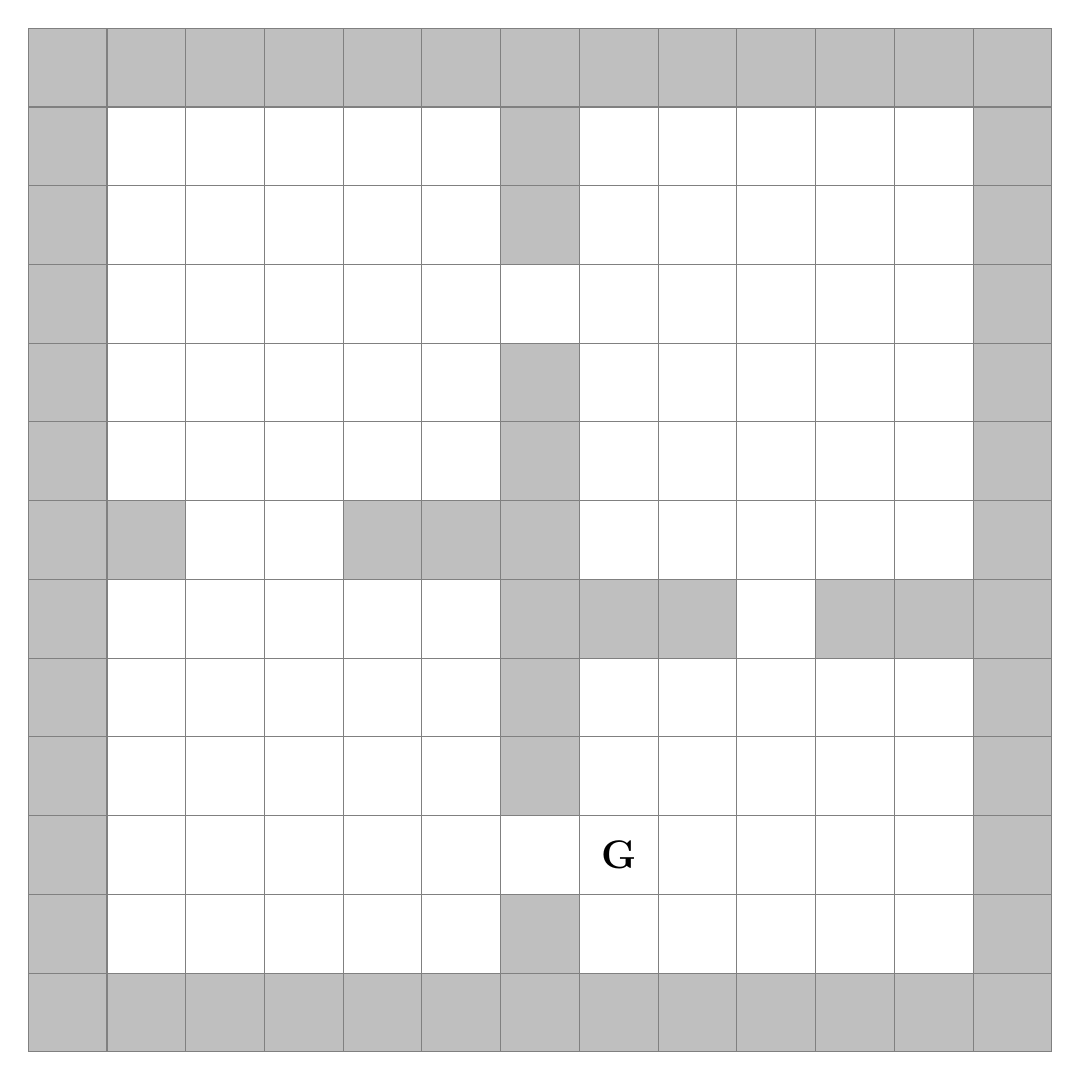
\begin{tikzpicture}[]
    % Darken walls
    % Boundaries
    \draw[fill=lightgray] (0,0) rectangle (1,13);
    \draw[fill=lightgray] (0,13) rectangle (13,12);
    \draw[fill=lightgray] (13,13) rectangle (12,0);
    \draw[fill=lightgray] (13,0) rectangle (0,1);

    % Room Borders
    \draw[fill=lightgray] (6,12) rectangle (7,10);
    \draw[fill=lightgray] (6,9) rectangle (7,3);
    \draw[fill=lightgray] (6,2) rectangle (7,1);

    \draw[fill=lightgray] (1,6) rectangle (2,7);
    \draw[fill=lightgray] (4,6) rectangle (6,7);

    \draw[fill=lightgray] (7,5) rectangle (9,6);
    \draw[fill=lightgray] (10,5) rectangle (12,6);

    % Grid
    \draw[step=1,color=gray] (0,0) grid (13,13);

    % Goal
%    \draw (1.5, 11.5) node { \Large{\bf S} };
    \draw (7.5, 2.5) node { \Large{\bf G} };

    % Option 1
    %\draw [o-latex, line width=2pt] (2.5,2.5) -- (2.5,1.5) -- (1.5,1.5);

    % Option 2
    %\draw [o-latex, line width=2pt] (2.5,3.5) -- (3.5,3.5) -- (3.5,4.5) -- (3.5,5.5);

    % Option 3
    %\draw [o-latex, line width=2pt] (3.5,5.5) -- (4.5,5.5) -- (5.5,5.5);

    % Option 4
    %\draw [o-latex, line width=2pt] (5.5,5.5) -- (5.5,4.5) -- (5.5,3.5) -- (5.5,2.3) -- (6.5,2.3) -- (7.5,2.3) -- (8.5,2.3) -- (9.7,2.3) -- (9.7,3.5) -- (9.7,4.5) -- (9.7,5.5) -- (9.7,6.5) -- (9.7,7.5) -- (9.7,8.5) -- (9.7,9.5) -- (9.5,9.5) -- (9.5,10.5);

    % Option 5
    %\draw [o-latex, line width=2pt] (11.5,11.5) -- (11.5,10.5) -- (11.5,9.5) -- (11.5,8.5);

    % Option 6
    %\draw [o-latex, line width=2pt] (11.5,8.5) -- (11.5,7.5) -- (10.5,7.5) -- (9.3,7.5) -- (9.3,6.5) -- (9.3,5.5) -- (9.3,4.5)  -- (8.5,4.5) -- (7.5,4.5) -- (7.5,3.5) -- (7.5,2.8);

    % Option 7
    %\draw [o-latex, line width=2pt] (1.5,7.5) -- (2.5,7.5) -- (2.5,6.5) -- (2.5,5.5) -- (2.5,4.5) -- (2.5,3.5) -- (2.5,2.7) -- (3.5,2.7) -- (4.5,2.7) -- (5.5,2.7) -- (6.5,2.7) -- (7.5,2.7) -- (8.5,2.7) -- (9.5,2.7);

    % Option 8
    %\draw [o-latex, line width=2pt] (9.5,4.5) -- (9.5,3.5)  -- (10.5,3.5); 

\end{tikzpicture}
\end{document}
